\documentclass{standalone}
\usepackage{tikz}
\usetikzlibrary{shapes,arrows,positioning,calc,patterns,backgrounds}

\begin{document}
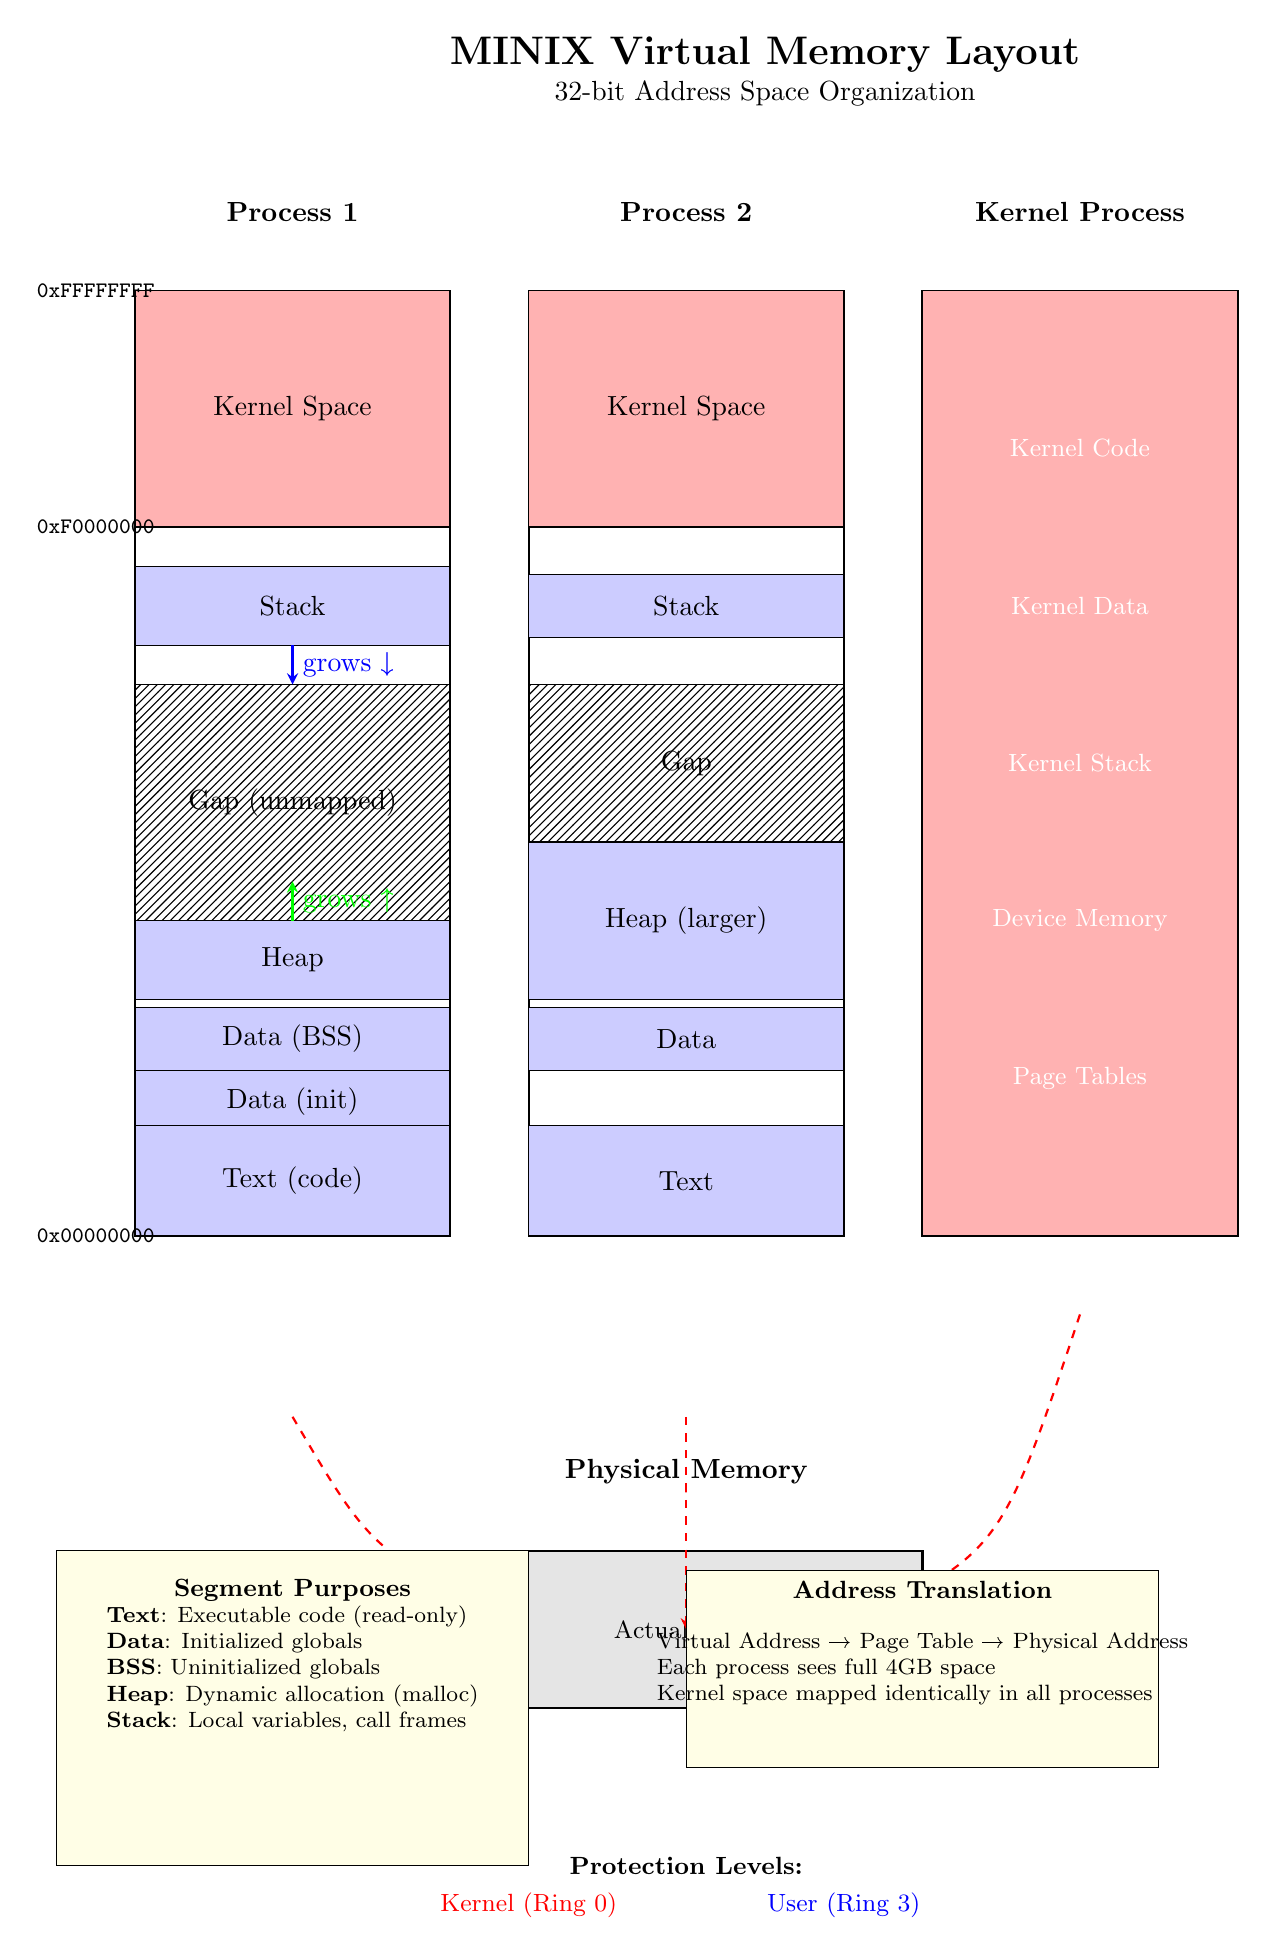
\begin{tikzpicture}[
    mem/.style={rectangle, draw=black, minimum width=4cm},
    kernel/.style={mem, fill=red!30},
    user/.style={mem, fill=blue!20},
    shared/.style={mem, fill=green!20},
    unused/.style={mem, fill=gray!10, pattern=north east lines},
    arrow/.style={->, >=stealth, thick},
    label/.style={font=\small},
    addr/.style={font=\footnotesize\ttfamily}
]

% Title
\node[font=\Large\bfseries] at (8, 15) {MINIX Virtual Memory Layout};
\node[font=\normalsize] at (8, 14.5) {32-bit Address Space Organization};

% Process 1 Memory Layout
\node[font=\bfseries] at (2, 13) {Process 1};
\draw[thick] (0, 0) rectangle (4, 12);

% Kernel space
\node[kernel, minimum height=3cm] (kern1) at (2, 10.5) {Kernel Space};
\node[addr] at (-0.5, 12) {0xFFFFFFFF};
\node[addr] at (-0.5, 9) {0xF0000000};

% User space sections
\node[user, minimum height=1cm] (stack1) at (2, 8) {Stack};
\node[unused, minimum height=3cm] (gap1) at (2, 5.5) {Gap (unmapped)};
\node[user, minimum height=1cm] (heap1) at (2, 3.5) {Heap};
\node[user, minimum height=0.8cm] (data1) at (2, 2.5) {Data (BSS)};
\node[user, minimum height=0.8cm] (init1) at (2, 1.7) {Data (init)};
\node[user, minimum height=1.4cm] (text1) at (2, 0.7) {Text (code)};
\node[addr] at (-0.5, 0) {0x00000000};

% Stack/Heap growth arrows
\draw[arrow, blue] (2, 7.5) -- node[right] {grows ↓} (2, 7);
\draw[arrow, green] (2, 4) -- node[right] {grows ↑} (2, 4.5);

% Process 2 Memory Layout (different process)
\node[font=\bfseries] at (7, 13) {Process 2};
\draw[thick] (5, 0) rectangle (9, 12);

% Kernel space (same mapping)
\node[kernel, minimum height=3cm] (kern2) at (7, 10.5) {Kernel Space};

% Different user layout
\node[user, minimum height=0.8cm] (stack2) at (7, 8) {Stack};
\node[unused, minimum height=2cm] (gap2) at (7, 6) {Gap};
\node[user, minimum height=2cm] (heap2) at (7, 4) {Heap (larger)};
\node[user, minimum height=0.8cm] (data2) at (7, 2.5) {Data};
\node[user, minimum height=1.4cm] (text2) at (7, 0.7) {Text};

% Kernel Process Layout
\node[font=\bfseries] at (12, 13) {Kernel Process};
\draw[thick] (10, 0) rectangle (14, 12);

% All kernel space
\node[kernel, minimum height=12cm] (kern3) at (12, 6) {};
\node[font=\small, white] at (12, 10) {Kernel Code};
\node[font=\small, white] at (12, 8) {Kernel Data};
\node[font=\small, white] at (12, 6) {Kernel Stack};
\node[font=\small, white] at (12, 4) {Device Memory};
\node[font=\small, white] at (12, 2) {Page Tables};

% Physical Memory Mapping
\begin{scope}[shift={(0, -3)}]
\node[font=\bfseries] at (7, 0) {Physical Memory};
\draw[thick, fill=gray!20] (4, -3) rectangle (10, -1);
\node[font=\small] at (7, -2) {Actual RAM};

% Mapping arrows
\draw[arrow, red, dashed] (2, 0.7) .. controls (3, -1) .. node[below] {MMU} (5, -2);
\draw[arrow, red, dashed] (7, 0.7) .. controls (7, -1) .. (7, -2);
\draw[arrow, red, dashed] (12, 2) .. controls (11, -1) .. (9, -2);
\end{scope}

% Memory segments explanation
\node[rectangle, draw=black, fill=yellow!10, minimum width=6cm, minimum height=4cm] at (2, -6) {};
\node[font=\small\bfseries] at (2, -4.5) {Segment Purposes};
\node[font=\footnotesize, align=left] at (2, -5.5) {
\textbf{Text}: Executable code (read-only)\\
\textbf{Data}: Initialized globals\\
\textbf{BSS}: Uninitialized globals\\
\textbf{Heap}: Dynamic allocation (malloc)\\
\textbf{Stack}: Local variables, call frames
};

% Virtual vs Physical annotation
\node[rectangle, draw=black, fill=yellow!10, minimum width=6cm, minimum height=2.5cm] at (10, -5.5) {};
\node[font=\small\bfseries] at (10, -4.5) {Address Translation};
\node[font=\footnotesize, align=left] at (10, -5.5) {
Virtual Address → Page Table → Physical Address\\
Each process sees full 4GB space\\
Kernel space mapped identically in all processes
};

% Protection rings indicator
\node[font=\small\bfseries] at (7, -8) {Protection Levels:};
\node[font=\small, red] at (5, -8.5) {Kernel (Ring 0)};
\node[font=\small, blue] at (9, -8.5) {User (Ring 3)};

\end{tikzpicture}
\end{document}